% File: basic_elements.tex
\documentclass{standalone}
\usepackage[american]{circuitikz}
\usepackage{cmbright}

\definecolor{myred}{RGB}{170,0,0}
\definecolor{myblue}{RGB}{0,0,220}

\ctikzset{bipoles/resistor/height=0.2}
\ctikzset{bipoles/resistor/width=0.5}

\begin{document}
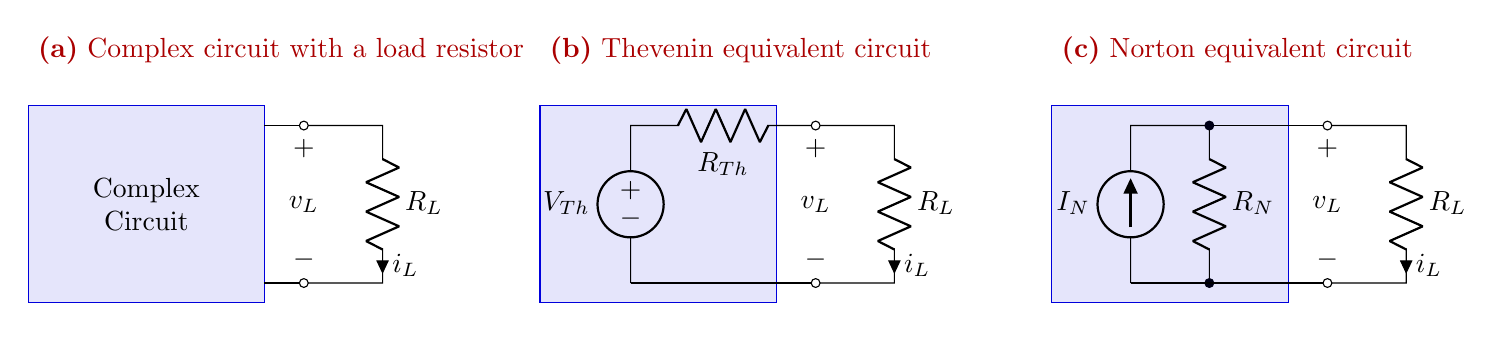
\begin{tikzpicture}
    % % Subtitle for the circuit.
    % \node[anchor=north west, font=\bfseries, color=myred] at (0, 3.25) {(b) Practical voltage source with a load resistor};
    % Complex circuit
    \begin{scope}
        % Subtitle for the circuit.
        \node[anchor=north west, color=myred, align=center] at (0, 3.25) {\textbf{(a)} Complex circuit with a load resistor};
        % Nodes A and B
        \draw (3.5, 2) node[ocirc] (A) {};
        \draw (A) node[right, yshift=3mm] {};
        \draw (3.5, 0) node[ocirc] (B) {};
        \draw (B) node[right, yshift=-3mm] {};

        % Complex circuit box.
        \draw[draw=myblue, fill=myblue, fill opacity=0.1, thin] (0, -0.25) rectangle (3, 2.25);
        % Text in the middle of the box.
        \node[anchor=center, color=black, align=center] at (1.5, 1) {Complex\\Circuit};

        % Voltage source and lower wire
        \draw (3, 2) to (A);
        \draw (3, 0) to (B);

        % Resistor and upper wire
        \draw (A) to ++(1, 0)
            to[R, l=$R_L$, i^>=$i_L$] ++(0, -2)
            to (B);

        % Voltage label across A and B
        \draw (A) to[open, v^=$v_{L}$] (B);
    \end{scope}

    % Thevenin equivalent circuit
    \begin{scope}[xshift=6.5cm]
        % Subtitle for the circuit.
        \node[anchor=north west, color=myred, align=center] at (0, 3.25) {\textbf{(b)} Thevenin equivalent circuit };
        % Nodes A and B
        \draw (3.5, 2) node[ocirc] (A) {};
        \draw (A) node[right, yshift=3mm] {};
        \draw (3.5, 0) node[ocirc] (B) {};
        \draw (B) node[right, yshift=-3mm] {};

        % Complex circuit box.
        \draw[draw=myblue, fill=myblue, fill opacity=0.1, thin] (0, -0.25) rectangle (3, 2.25);

        % Voltage source and lower wire
        \draw (1.15, 0) to[V, l={$V_{Th}$}, invert] (1.15, 2) to[R, l_=$R_{Th}$] (A);
        \draw (1.15, 0) -- (B);

        % Resistor and upper wire
        \draw (A) to ++(1, 0)
            to[R, l=$R_L$, i^>=$i_L$] ++(0, -2)
            to (B);

        % Voltage label across A and B
        \draw (A) to[open, v^=$v_{L}$] (B);
    \end{scope}

    % Norton equivalent circuit
    \begin{scope}[xshift=13cm]
        % Subtitle for the circuit.
        \node[anchor=north west, color=myred, align=center] at (0, 3.25) {\textbf{(c)} Norton equivalent circuit };
        % Nodes A and B
        \draw (3.5, 2) node[ocirc] (A) {};
        \draw (A) node[right, yshift=3mm] {};
        \draw (3.5, 0) node[ocirc] (B) {};
        \draw (B) node[right, yshift=-3mm] {};
        \draw (2.0, 2) node[circ] (C) {};
        \draw (2.0, 0) node[circ] (D) {};

        % Complex circuit box.
        \draw[draw=myblue, fill=myblue, fill opacity=0.1, thin] (0, -0.25) rectangle (3, 2.25);

        % Voltage source and lower wire
        \draw (1.0, 0) to[I, l={$I_{N}$}] (1.0, 2) to (C) to[R, l=$R_{N}$] (D);
        \draw (1.0, 0) -- (B);
        \draw (C) to (A);

        % Resistor and upper wire
        \draw (A) to ++(1, 0)
            to[R, l=$R_L$, i^>=$i_L$] ++(0, -2)
            to (B);

        % Voltage label across A and B
        \draw (A) to[open, v^=$v_{L}$] (B);
    \end{scope}

    % % Plot of v_L vs i_L (top right)
    % \begin{scope}[xshift=4cm]
    %     % Axes
    %     \draw[->] (0, 0) -- (0, 2) node[left] {$v_L$};
    %     \draw[->] (0, 0) -- (4, 0) node[below] {$i_L$};
    %     % Plot
    %     \begin{scope}
    %         % vl = v_s - i_L * R_s
    %         \clip (0, 0) rectangle (4, 2);
    %         \draw[ultra thick, myred] (-0.1, 1.5) -- (3.5, -0.1);
    %     \end{scope}
    % \end{scope}
\end{tikzpicture}
\end{document}